\section{Modelado del Sistema}

\subsection{Diagrama de Casos de Uso}
\label{sec:casos_uso}

Para definir claramente las interacciones entre los distintos tipos de usuarios y el portal web, se elaboró un diagrama de casos de uso (véase la Figura \ref{fig:casos_uso}). Este esquema permite visualizar las acciones que puede realizar un usuario público (como la consulta de noticias, mapas interactivos y oferta educativa) en contraste con las capacidades de gestión del administrador del sistema.

\begin{figure}[!tbh]
    \centering
    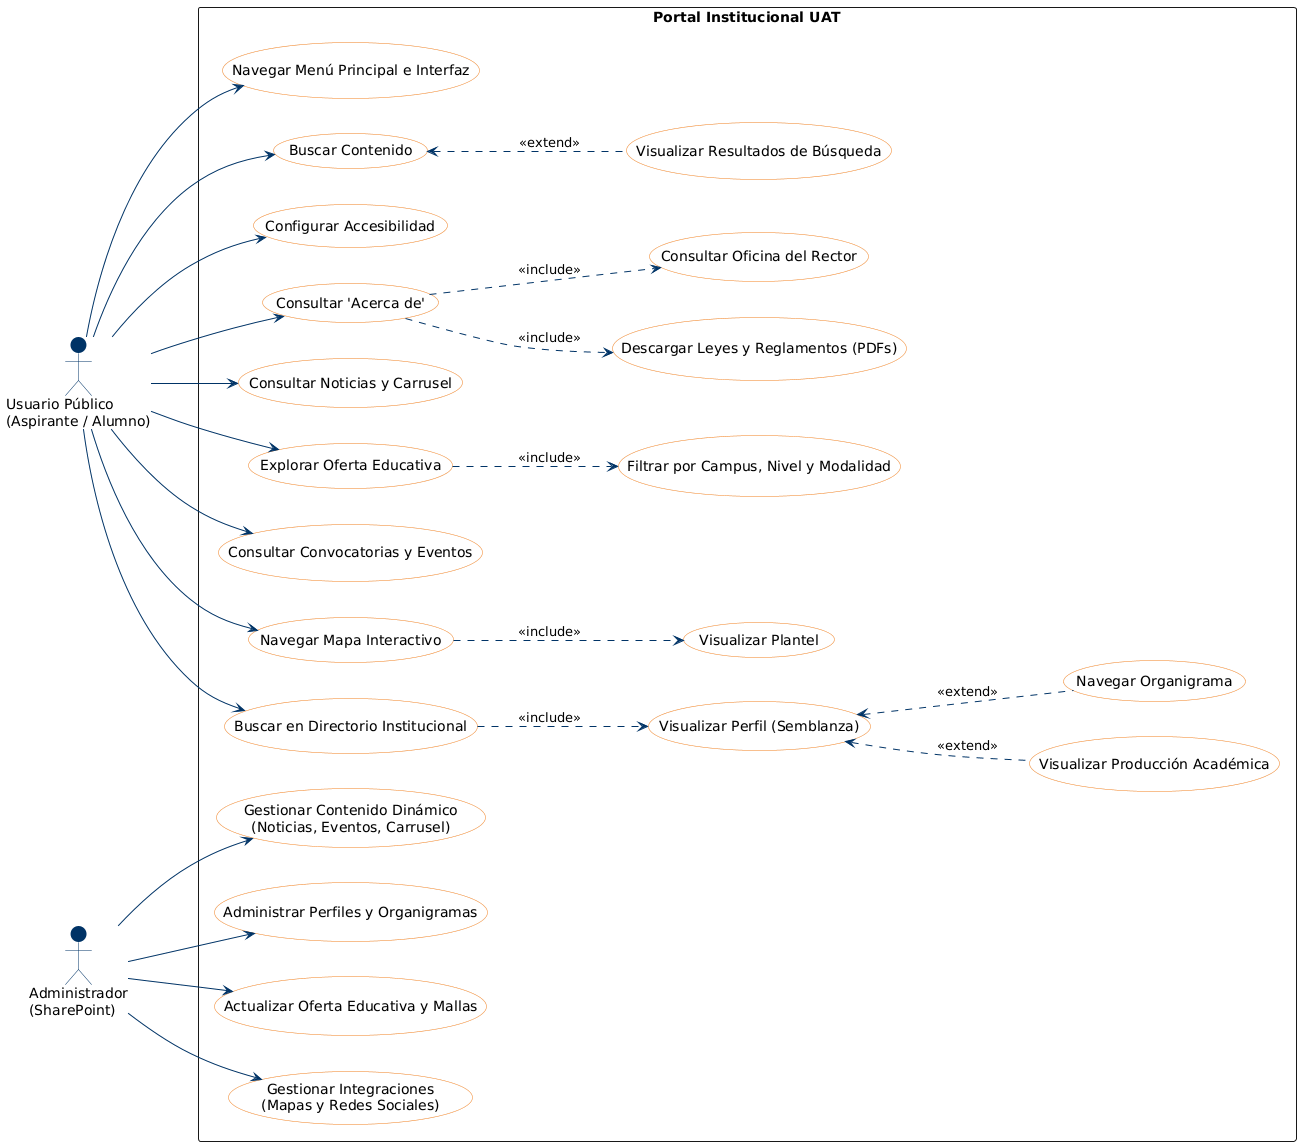
\includegraphics[width=0.9\linewidth]{img/Diagrama_casos_uso.png}
    \caption{Diagrama de Casos de Uso del Portal Institucional}
    \label{fig:casos_uso}
\end{figure}

\subsection{Modelo Relacional de Base de Datos}
\label{sec:base_datos}

Para garantizar la integridad y correcta gestión de la información dinámica del portal (como las noticias, el directorio del personal y la oferta educativa), se diseñó un modelo relacional de base de datos. Como se observa en la Figura \ref{fig:base_datos}, el modelo fue normalizado para evitar la redundancia de datos, separando entidades clave y estableciendo las relaciones necesarias mediante llaves primarias y foráneas.

\begin{figure}[!tbh]
    \centering
    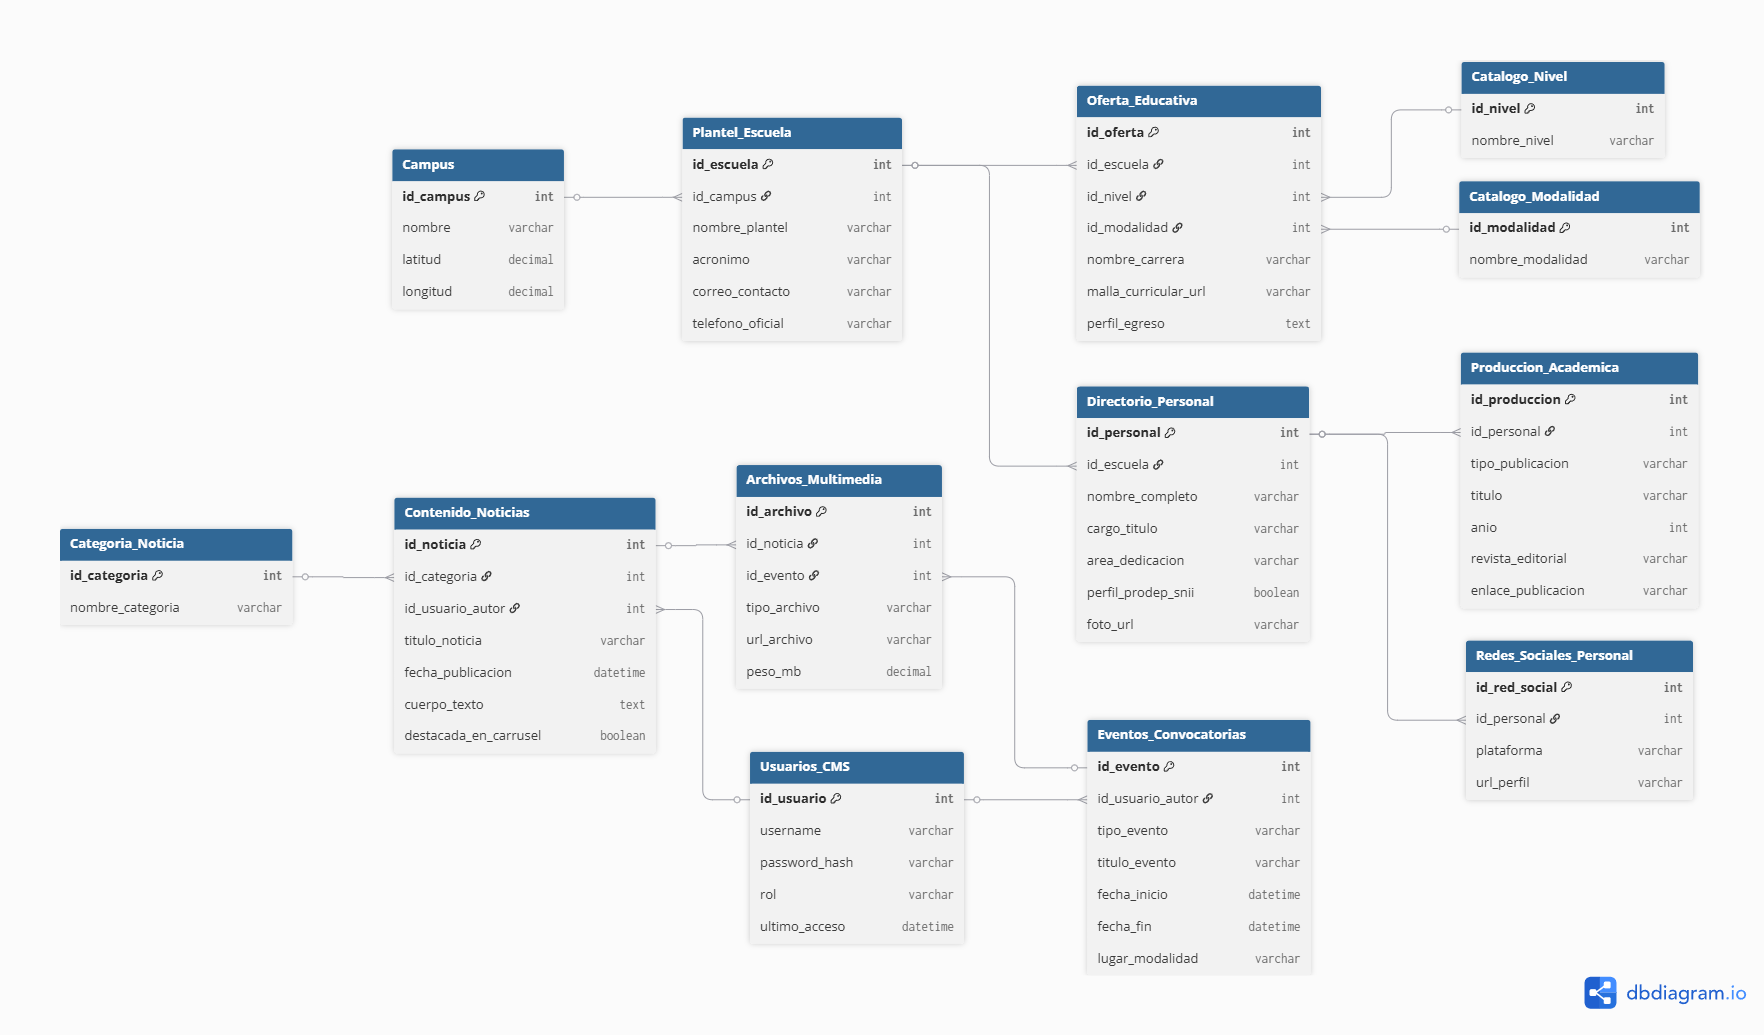
\includegraphics[width=\linewidth]{img/Diagrama_base_datos.png}
    \caption{Modelo Entidad-Relación de la Base de Datos}
    \label{fig:base_datos}
\end{figure}

\clearpage
\subsection{Diagramas de Actividades}
\label{sec:actividades}

Para detallar los procesos principales que el usuario realiza dentro de la plataforma, se diseñaron tres diagramas de actividades. En primer lugar, la Figura \ref{fig:actividad3} expone el consumo asíncrono de contenidos en la página de inicio, demostrando la integración simultánea de noticias internas con las interfaces de programación de aplicaciones (API) de redes sociales. En la Figura \ref{fig:actividad1}, se describe el flujo de navegación para la consulta de oferta educativa, ilustrando cómo el sistema filtra las opciones hasta permitir la descarga de la malla curricular. Finalmente, la Figura \ref{fig:actividad2} muestra la interacción con el mapa interactivo del campus, detallando la carga de coordenadas y la visualización de datos en componentes dinámicos.

\begin{figure}[!hbt]
    \centering
    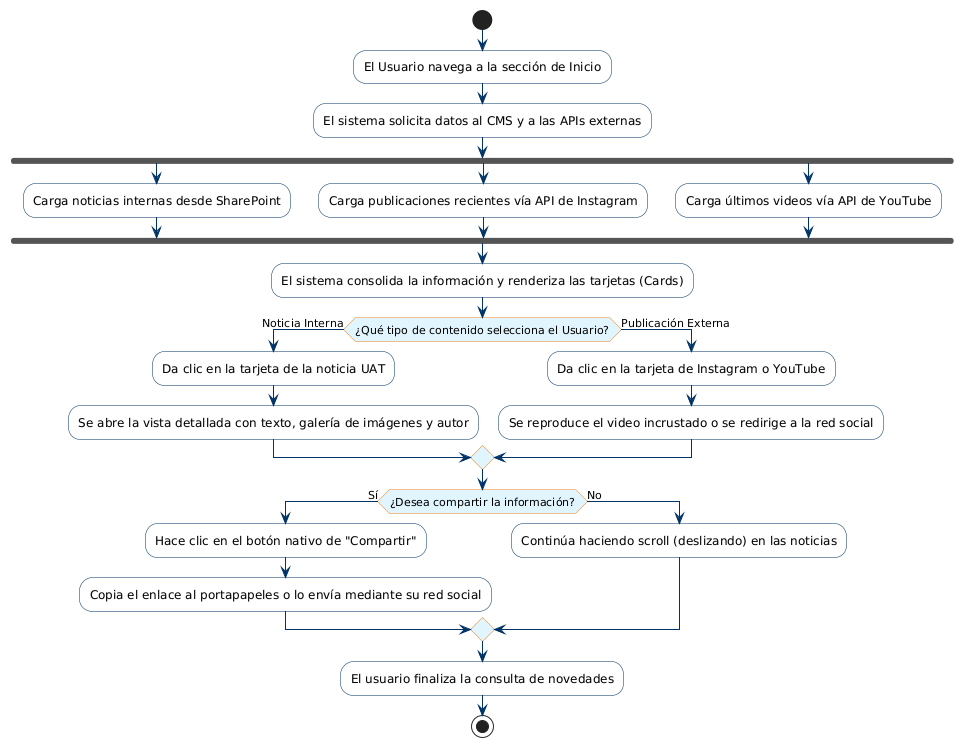
\includegraphics[width=0.85\linewidth]{img/Diagrama_Actividad_3.png}
    \caption{Diagrama de Actividades: Consumo de Noticias y Redes Sociales}
    \label{fig:actividad3}
\end{figure}

\begin{figure}[!hbt]
    \centering
    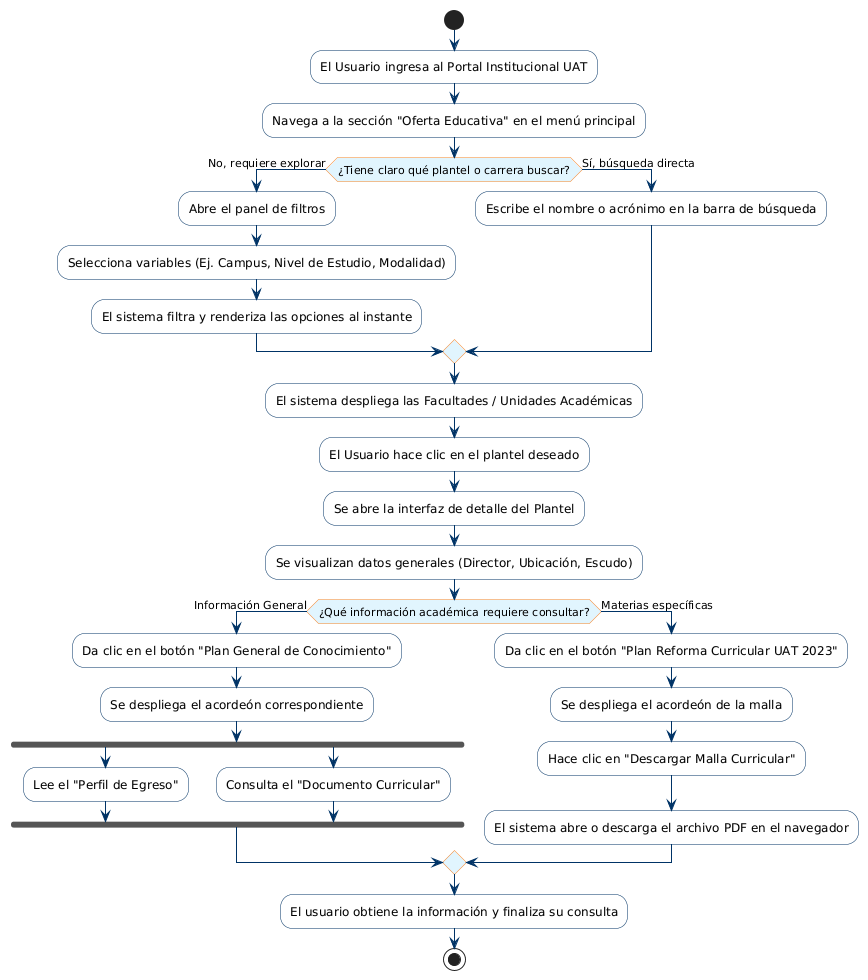
\includegraphics[width=\linewidth]{img/Diagrama_Actividad_1.png}
    \caption{Diagrama de Actividades: Consulta de Oferta Educativa}
    \label{fig:actividad1}
\end{figure}

\begin{figure}[!hbt]
    \centering
    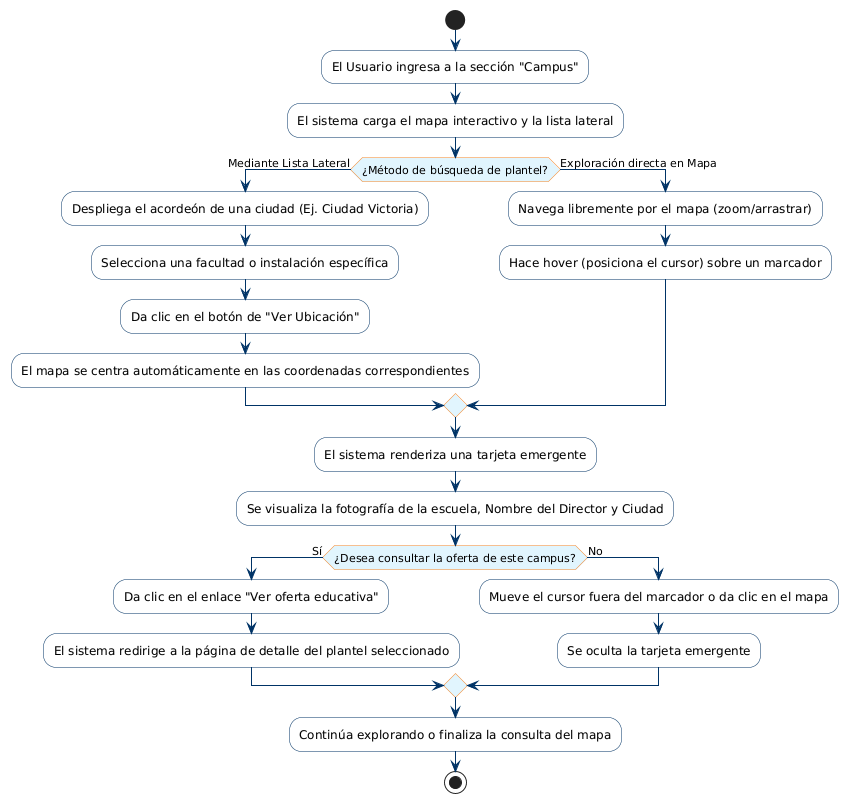
\includegraphics[width=0.9\linewidth]{img/Diagrama_Actividad_2.png}
    \caption{Diagrama de Actividades: Navegación del Mapa Interactivo}
    \label{fig:actividad2}
\end{figure}

\clearpage
\subsection{Diagramas de Secuencia}
\label{sec:secuencia}

Para establecer la comunicación técnica entre la interfaz de usuario, el servidor y la base de datos, se elaboraron diagramas de secuencia enfocados en los módulos de mayor complejidad. La Figura \ref{fig:secuencia1} ilustra el proceso del motor de búsqueda general, evidenciando las validaciones del lado del cliente y el manejo de respuestas en formato JSON. Asimismo, la Figura \ref{fig:secuencia2} detalla el flujo de consulta del directorio institucional, graficando las peticiones realizadas para la carga inicial de áreas y la filtración específica de perfiles.

\begin{figure}[!hbt]
    \centering
    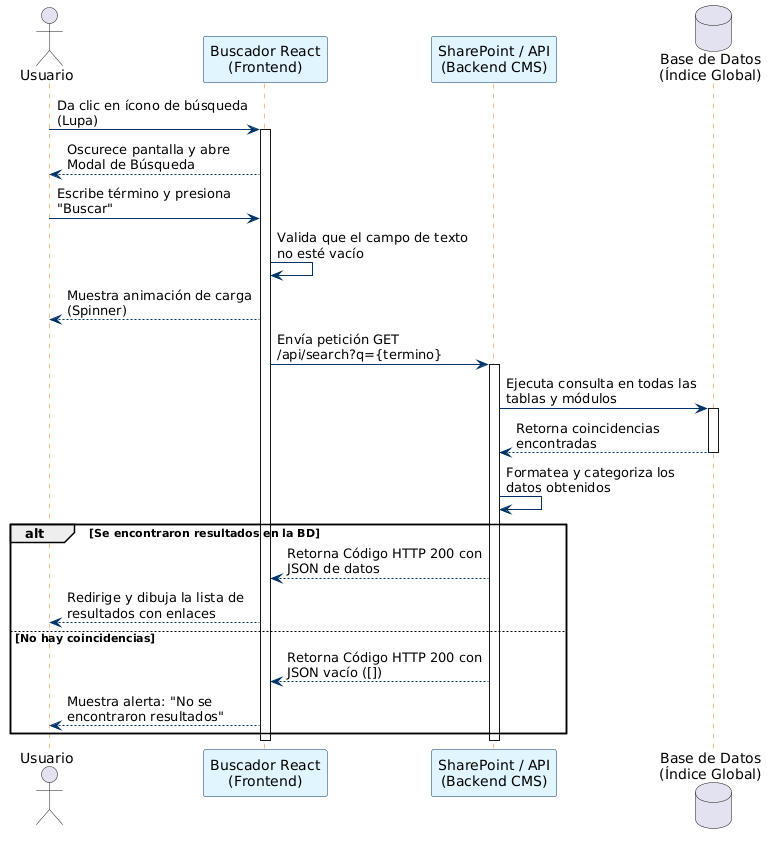
\includegraphics[width=0.8\linewidth]{img/Diagrama_Secuencia_1.png}
    \caption{Diagrama de Secuencia: Motor de Búsqueda General}
    \label{fig:secuencia1}
\end{figure}

\begin{figure}[!hbt]
    \centering
    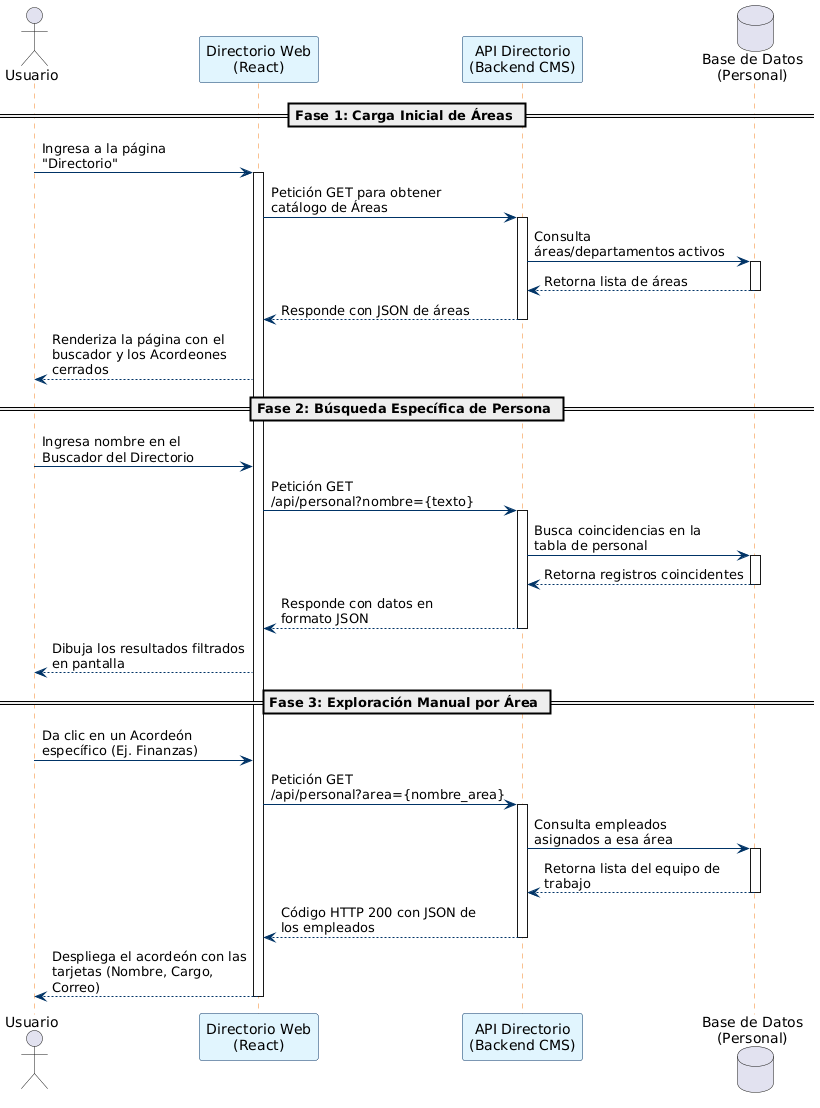
\includegraphics[width=0.9\linewidth]{img/Diagrama_Secuencia_2.png}
    \caption{Diagrama de Secuencia: Consulta de Directorio Institucional}
    \label{fig:secuencia2}
\end{figure}
